\chapter{Theoretical background}

\section{Natural language morphology and typology}

\subsection{What is natural language morphology?}

One way that human languages express grammatical or semantic meaning is by altering individual words; this process is called \textbf{morphology}. Linguistic morphology is split into two major categories: \textbf{inflectional} and \textbf{derivational}. Inflectional morphology comprises alterations to words that reflect \textit{grammatical} meaning, that is, it indicates which of a determined subset of grammatical categories is at work in a particular phrase. For example, the verb \textit{paint} is grammatically inflected in the sentence \textit{"He paints."} to indicate agreement with a third-person singular subject. Derivational morphology applies \textit{semantic} alterations, that is, it shifts the fundamental meaning of a word, often switching its part of speech. For example, the verb \textit{paint} can become the noun \textit{painter}, denoting a person characterized by performing the action of the verb \parencite{Hogan2010}. 

The concept of \textbf{part of speech} refers to high-level groupings of words within a language according to what inflectional morphology they may undergo. Common parts of speech include nouns, verbs, and adjectives, although the exact division of parts of speech is language-specific. Within a given language and part of speech, there is typically a well-defined, finite set of \textbf{forms} that a given word may take; that abstract set of forms is called a \textbf{paradigm}. In particular, there is typically a set of \textbf{morphological categories} associated with a given part of speech in a given language. Common examples of morphological categories include number (e.g., singular vs. plural), verb tense, and noun or pronoun case (English exhibits case only in pronouns: I, me, my). Inflection is then used to assign a value to some or all of the morphological categories for a given word \parencite{Hogan2010}. For example, Spanish adjectives such as \textit{pequeño} "small" inflect for gender and number:

\begin{center}
\begin{tabular}{|c||c|c|}
\hline
& singular & plural \\
\hline \hline
masculine & \textit{pequeño} & \textit{pequeños} \\
\hline 
feminine & \textit{pequeña} & \textit{pequeñas} \\
\hline
\end{tabular}
\end{center}

 The term "word" can be ambiguous when speaking of linguistic morphology. To be more specific, a \textbf{form} is a word with a specific spelling or pronunciation and corresponding to a specific set of grammatical values, e.g., a single cell in the above table. The set of forms across an entire inflectional paradigm are said to belong to the same \textbf{lexeme}. A lexeme can be identified by its \textbf{lemma} - a citation or dictionary form, a particular cell in the paradigm that is chosen to represent the entire lexeme. Spanish adjectives are usually cited in the masculine singular, so the above forms may be said to belong to the Spanish lexeme that has the lemma \textit{pequeño} \parencite{Hogan2010}.

In contrast, derivational morphology is applied in a less systematic manner, and constraints on its application are as often semantic or idiosyncratic as determined by part of speech or other formal categories. For example, the English verb \textit{like} may become the common derived term \textit{likeable}, but an analogous term \textit{hateable} is much less often seen. For this reason, derivational morphology is more difficult to systematically study; this paper is only concerned with inflectional morphology.

An important concept in morphology is that of \textbf{inflection classes} - subgroupings of parts of speech in a given language that exhibit similar patterns of inflection to one another. An example the division of Spanish verbs into \textit{-ar}, \textit{-er}, and \textit{-ir} classes:

\begin{center}
\begin{tabular}{|c|c|c|c|}
\hline
infinitive & 3rd person sg. imperfect indicative & gerund \\
\hline \hline
\textit{bailar} & \textit{bailaba} & \textit{bailando} \\
\hline 
\textit{comer} & \textit{comía} & \textit{comiendo} \\
\hline 
\textit{partir} & \textit{partía} & \textit{partiendo} \\
\hline 
\end{tabular}
\end{center}

Many types of grammatical categories commonly appear cross-linguistically, such as number, gender, animacy, case, politeness, tense, aspect, mood, and definiteness. The values that these categories may take often differ somewhat in meaning from language to language (for instance, English only has one inflected past tense while Spanish has two), but the parallels between them are typically enough that it's possible to make general characterizations of the degree of similarity of inflection systems between to languages. English and Spanish both inflect nouns for singular and plural number, and neither inflects nouns for case, but Spanish can inflect some human nouns for gender as well, and inflects adjectives for number and gender where English adjectives are not \parencite{Hogan2010}. A related notion is that of paradigm size. English nouns only ever take two forms - singular and plural - while Finnish nouns may take about 28 \parencite{Wiktionary}.

\subsection{Types of inflection}

There are many \textbf{inflection shapes} seen in natural languages. The most basic is \textbf{affixation}: the addition of sounds to the beginning, middle, or end of a word. Affixation can be broadly divided into prefixation (addition of an affix to the beginning of a word), suffixation (to the end), infixation (in the middle), circumfixation (at both ends). Other designations for affixation shapes include ablaut (alteration or replacement of a sound in the middle of a word) and templatic morphology. Templatic morphology is a complex process by which certain elements of a stem are distributed throughout a form, interwoven with elements indicating grammatical value. 

\textbf{Fusion} refers to the marking of multiple categories at once with a single indivisible morpheme, e.g., the Spanish verb \textit{hablé} "I spoke" marks tense and subject person and number with the suffix \textit{-é}, lacking separable morphemes to indicate the preterite tense and first person singular subject (cf. \textit{hablo} "I speak", \textit{habló} "he/she spoke"). 

\begin{center}
\begin{tabular}{|c||c|c|}
\hline
& 1st person singular & 3rd person singular \\
\hline \hline
present & \textit{hablo} & \textit{habla} \\
\hline 
preterite & \textit{hablé} & \textit{habló} \\
\hline
\end{tabular}
\end{center}

\textbf{Reduplication} is the repetition of all or part of a word. Reduplication may be full, as in Indonesian \textit{orang} "person" vs. \textit{orang-orang} "people", or partial, as in the formation of the contemplative aspect of the Tagalog word \textit{bili} "buy" by repeating the first syllable: \textit{bibili} (examples from Wiktionary). 

\textbf{Long-distance morphophonological processes} are those by which the surface form of an affix depends on the phonological properties of a segment at some distance from the affixation site. For instance, Finnish exhibits vowel harmony, a process by which the vowels present in affixes depend on the set of vowels in the stem. The Finnish inessive singular suffix \textit{-ssa/-ssä} looks different on the nouns \textit{puku} "suit" and \textit{kenkä} "shoe", with the final vowel of the suffix dependent on the set of vowels in the rest of the word. 

\begin{center}
\begin{tabular}{|c|c|}
\hline
nominative singular & inessive singular \\
\hline \hline
\textit{puku} & \textit{puvussa} \\
\hline 
\textit{kenkä} & \textit{kengässä} \\
\hline
\end{tabular} \\
\vspace{.3cm}
\parencite{Wiktionary}
\end{center}

Lastly, \textbf{irregularity} is a concept with familarity to anyone who's ever tried to learn a foreign language. Forms or entire lexemes are said to be irregular if they are aberrant from the normal patterns of morphology. For example, almost all English verbs only mark a third person singular subject differently from others, with a suffix \textit{-s}: \textit{I run} but \textit{she runs}. However, \textit{to be} marks the first person singular subject differently as well, and the third person singular subject marking bears no resemblance to the normal affixation process: \textit{I am}, \textit{you are}, \textit{she is}. It can be said that \textit{be} is a highly irregular verb.

\subsection{Linguistic typology}

\textbf{Linguistic typology} refers to the classification of languages into different categories depending on their structure. The major categories of morphological typology are \textbf{isolating}, \textbf{agglutinating}, and \textbf{fusional}. Languages are considered to be more isolating if they have little grammatical inflection, smaller inflection paradigms, and a smaller number of affixes per word on average \parencite{Hogan2010}. English is a fairly isolating language, likely a factor in the lack of computational morphology research \parencite{Cotterell2017}. Languages are considered to be more agglutinating if they exhibit more extensive inflection but do not typically exhibit fusion; agglutination is also associated with greater morphological regularity. Fusional languages are simply those that exhibit relatively more fusion. Like many typological distinctions, there is no strict assignment of languages into one or another of these categories; rather, they are ends of a spectrum that languages may be placed along \parencite{Hogan2010}.

Other typological labels may be applied depending on the set and shape of morphological inflection. Languages may be considered \textbf{highly inflecting} or \textbf{polysynthetic} if they have very large morphological paradigms. Languages may be typified by the presence of grammatical gender, vowel harmony, or other morphological characteristics. In general, this study is not concerned with defining specific labels for languages so much as computationally measuring the structural similarity of their morphological systems.

\subsection{Linguistic genealogy}

\begin{figure}[ht]
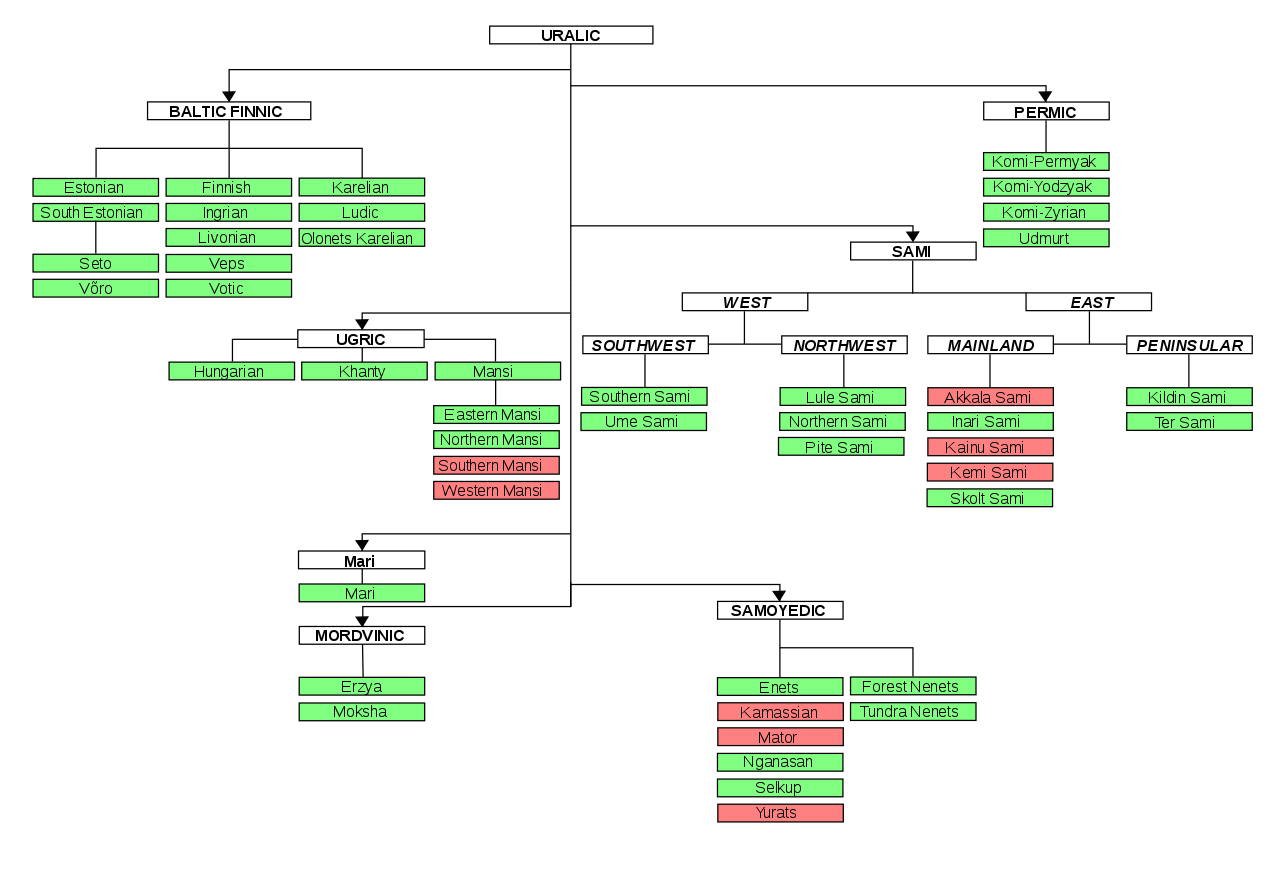
\includegraphics[width=13cm]{images/1280px-UralicTree.png}
\centering
\caption{The entire Uralic language family. \\ (commons.wikimedia.org/wiki/File:UralicTree.svg)}
\end{figure}

Languages change and diverge over time, and their development tends to follow genealogical patterns analogous to species descent and divergence. They are commonly grouped into \textbf{language families}, described with genealogical trees, and genealogical distance can be measured between them.

Language relationships are ascertained via historical comparison, and language families are simply the largest possible groupings that can be supported with certainty by available evidence. As such, they are not alike in historical timescale or internal diversity; more well-studied or attested families, and those with more historical written material, are likely to be larger because there is information available with which to make inferences about language descent in the distant past.

For this reason, a simple measure of genealogical separation cannot easily be come by. Relative location in a language family tree may not be informative, since the number of members and the density of branching differs between families. Another strategy is to measure \textbf{lexical similarity}: the proportion of words between two languages which are obviously similar due to shared origin.

However, lexical similarity is a measure of the similarity of vocabulary items and is not a good proxy for the grammatical similarity of languages. English has borrowed a very large amount of vocabulary from various historical varieties of French, yet their morphological systems remain fairly faithful to their respective origins in different branches of the Indo-European family. French in particular bears substantial morphological similarity to other Western Romance languages like Spanish and Portuguese. Even languages with no known genealogical relationship and extremely different grammatical systems may have non-zero lexical similarity: Turkish and Urdu have both borrowed heavily from Arabic, yet the grammatical systems of the three languages are quite distinct.

\section{LSTM and GRU neural modeling}
\label{sec:LSTM}

\begin{figure}[p]
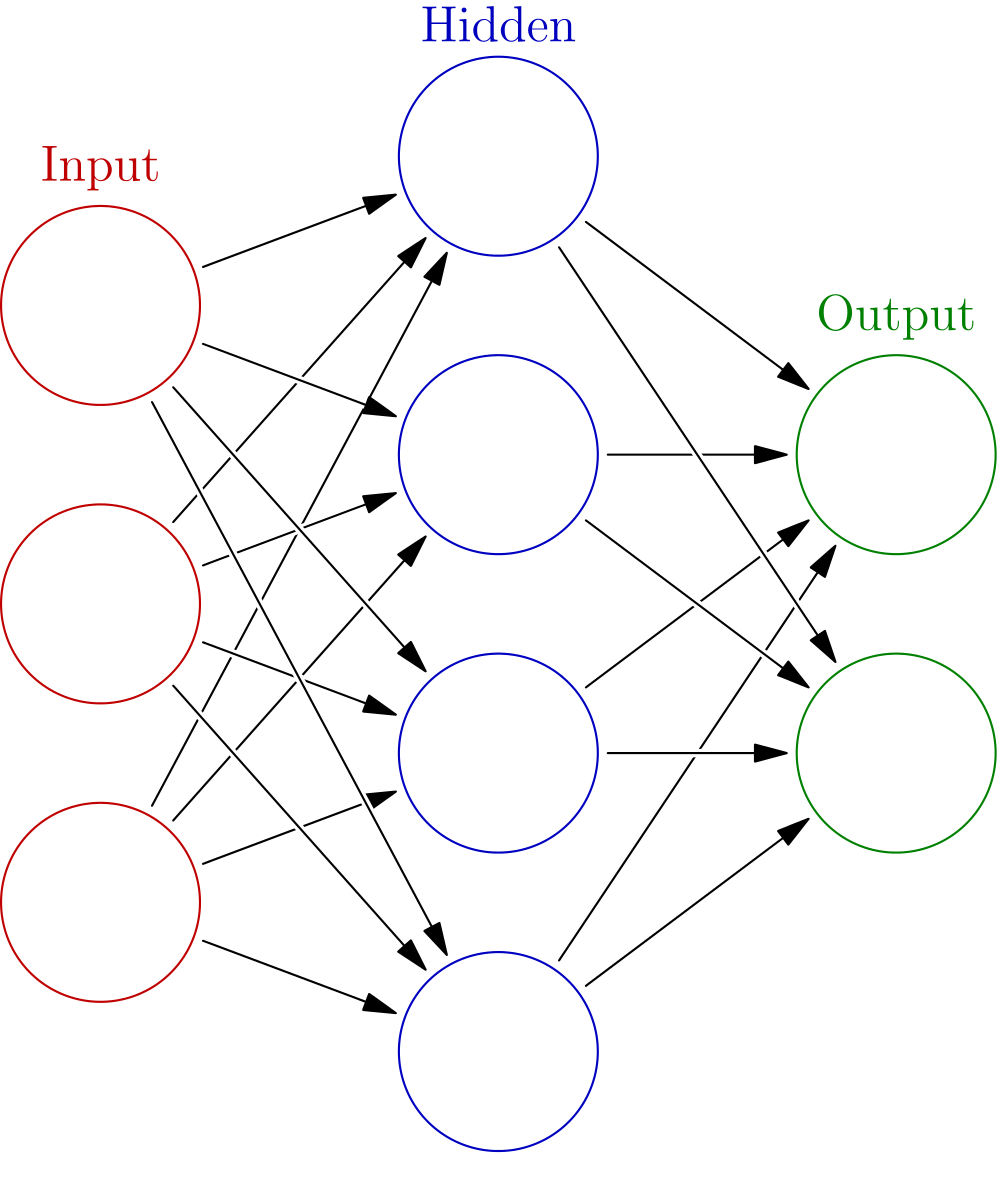
\includegraphics[width=6cm]{images/1000px-Colored_neural_network.png}
\centering
\caption{The structure of a feed-forward neural network with three inputs, four hidden cells, and two outputs. \\ (commons.wikimedia.org/wiki/File:Colored\_neural\_network.svg)}
\label{fig:NN}
\end{figure}

\begin{figure}[p]
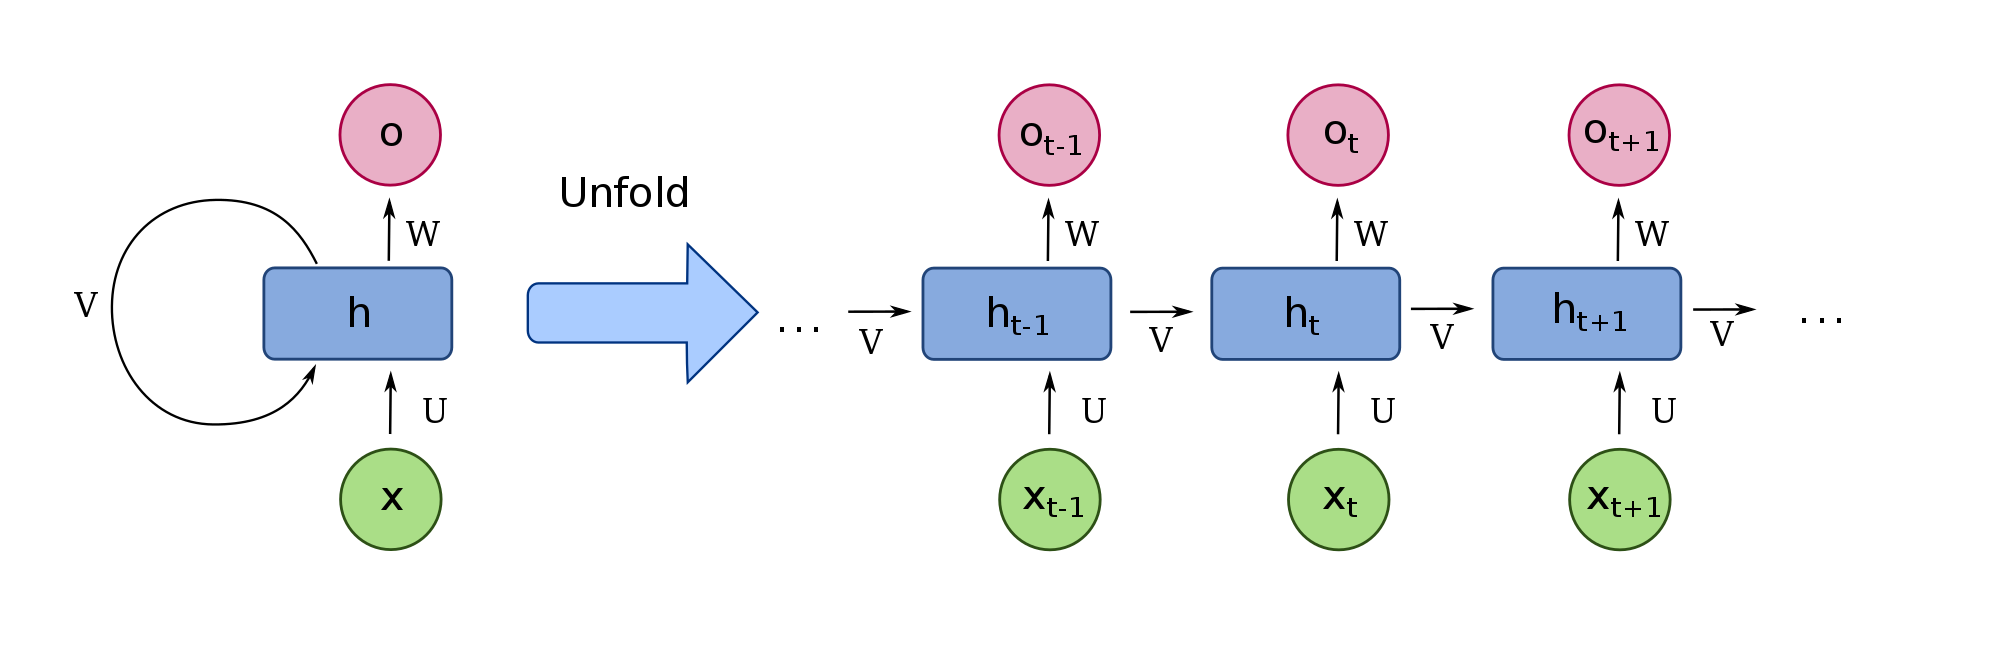
\includegraphics[width=12cm]{images/RNN.png}
\centering
\caption{The generalized structure of a recurrent neural network. \\ (commons.wikimedia.org/wiki/File:Recurrent\_neural\_network\_unfold.svg)}
\label{fig:RNN}
\end{figure}

\begin{figure}[p]
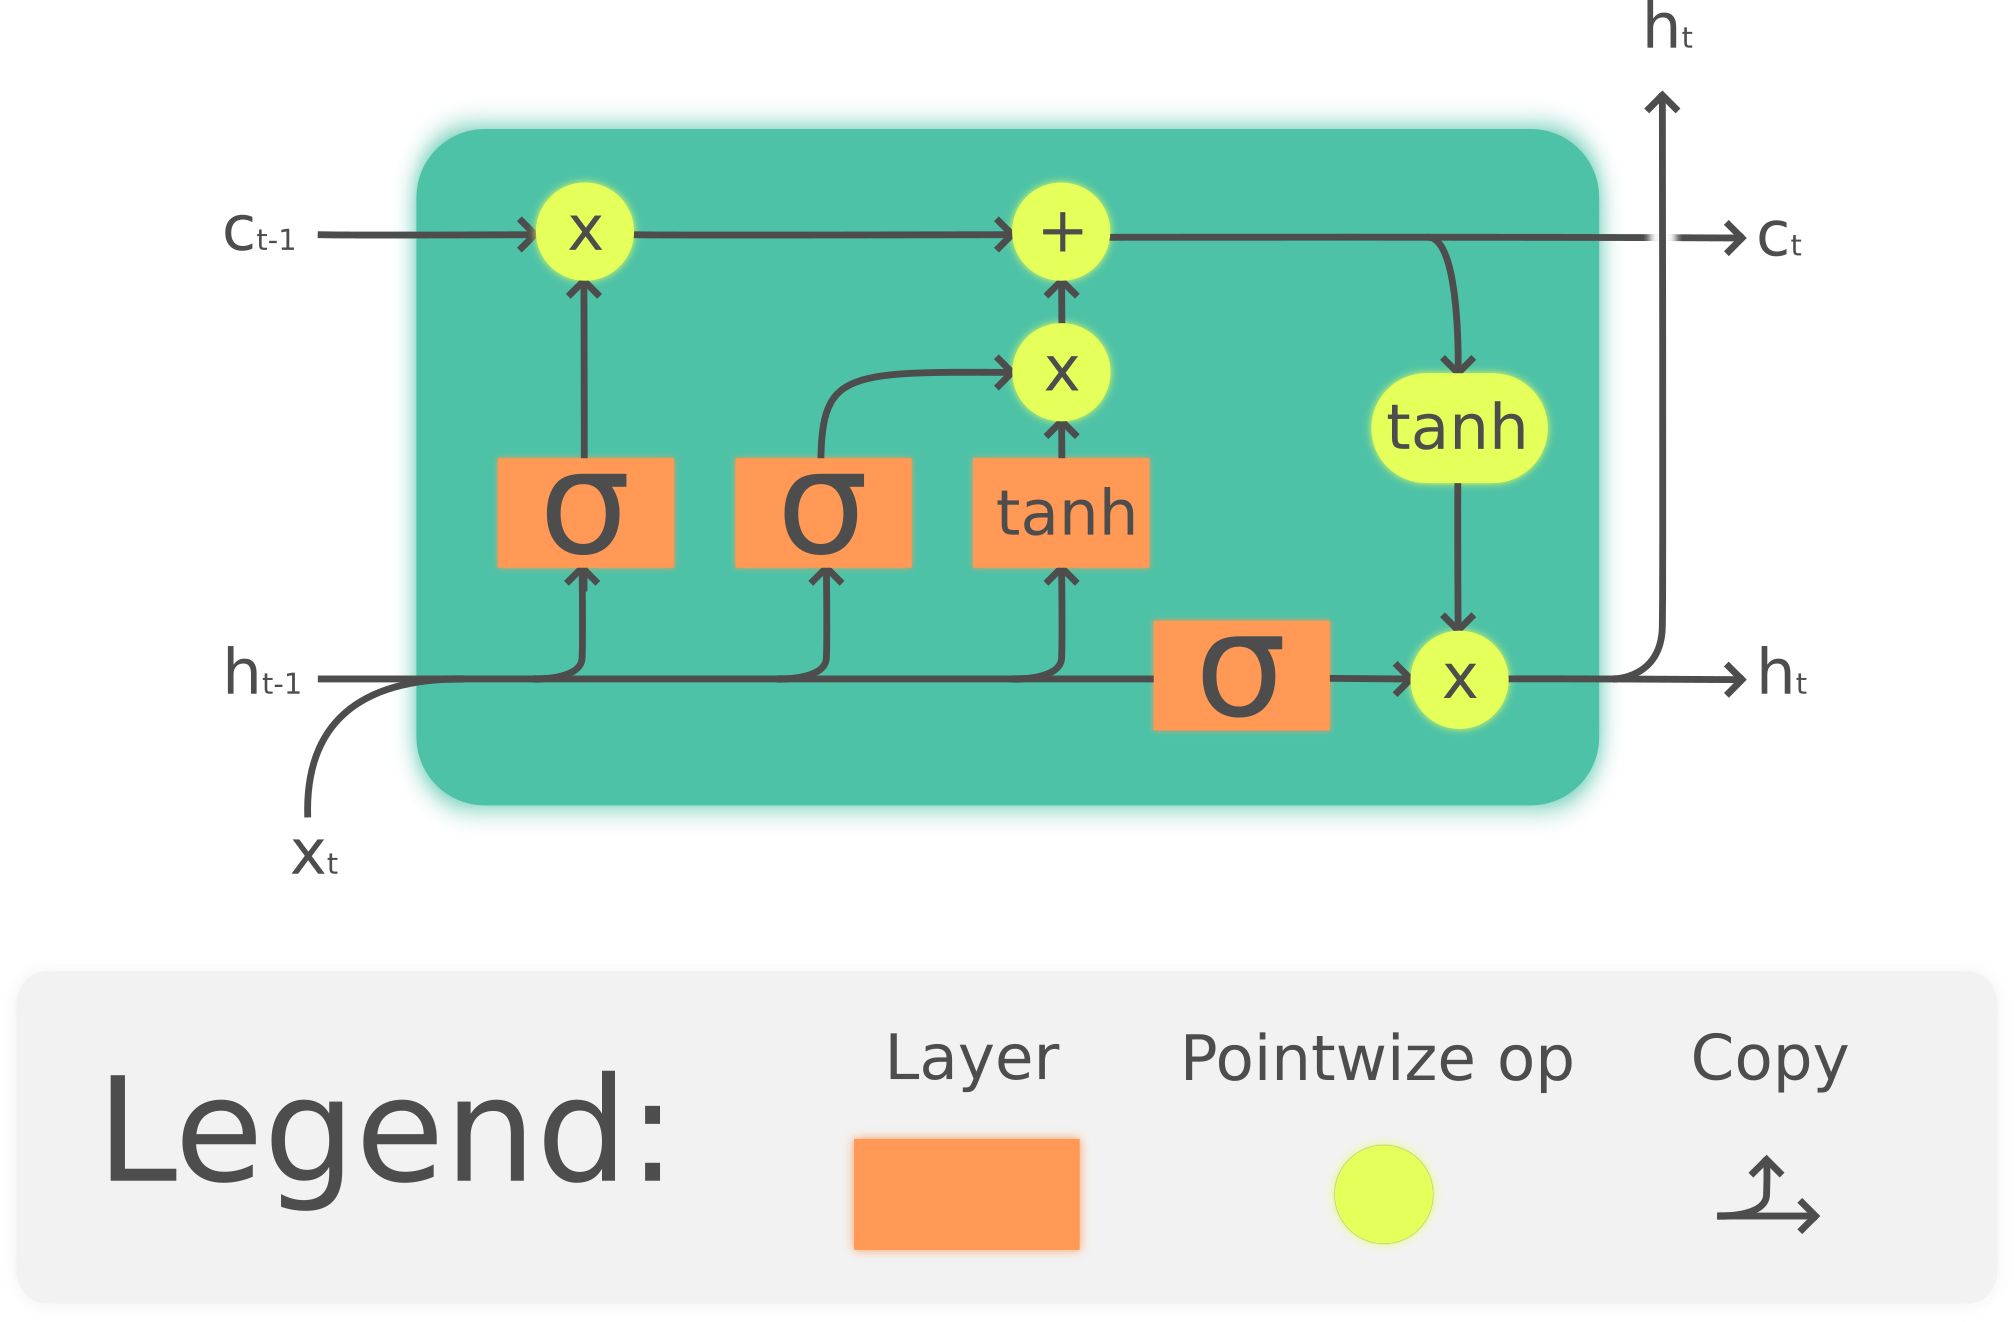
\includegraphics[width=12cm]{images/The_LSTM_cell.png}
\centering
\caption{The state cell of an LSTM model. \\ (commons.wikimedia.org/wiki/File:The\_LSTM\_cell.png)}
\label{fig:LSTM}
\end{figure}

\textbf{Neural networks} are a type of function approximation model inspired by the connection of neurons in animal brains. They have come to be implemented in a variety of forms, and underlie state of the art machine learning models in a variety of applications. The common feature of neural models is repeated matrix multiplication followed by the application of a non-linear "activation" function. Fig. \ref{fig:NN} illustrates a simple feed-forward network, in which a vector of three inputs is multiplied by some $3 \times 4$ matrix and activated to produce a vector of four intermediate values, which are again multiplied by some $4 \times 2$ matrix and activated to produce a vector of two outputs.

A \textbf{recurrent neural network (RNN)} is a type of neural network that operates over sequences of inputs, typically with unknown length. Fig. \ref{fig:RNN} illustrates the general structure: each input is represented by a vector, which is multiplied by a vector $U$ to modify state, and the modified state is then multiplied by a vector $W$ to produce an output vector and a matrix $V$ to produce the next state. 

\textbf{Long short-term memory (LSTM)} neural networks are a variant of RNNs which use a more complex sequence of computations to update state, and maintain a separate piece of state \textit{c} that controls rate of forgetting. LSTMs are intended to solve the forgetfulness of more basic RNN types, which tend to be unable to recall information from more than a few iterations prior \parencite{Hochreiter1997}. LSTM architecture is described in Fig. \ref{fig:LSTM}: the input $x_i$ and the previous state $h_{i-1}$ are linearly transformed, added, and activated, as in a simple RNN, before interacting via a series of operations with the previous cell $c_{i-1}$, producing the next state $h_i$ and cell $c_i$. \textbf{Gated recurrent units} (GRU) are slightly simplified models that do not include separate parameterization of the output gate (not pictured).

LSTMs have become the dominant model type in a variety of language tasks, including syntactic and morphological tasks. They significantly outperformed other types of models in SIGMORPHON 2016, since which time they have come to underlie nearly all morphology prediction models (\cite{Cotterell2016}, \cite{Cotterell2017a}).

\begin{figure}[ht]
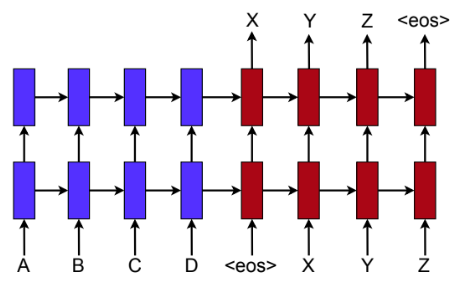
\includegraphics[width=10cm]{images/stacked.png}
\centering
\caption{A stacked RNN architecture, in which there are two layers of hidden state. In this architecture, hidden states in the second layer are exclusively derived from the aligned cell of the first layer. \parencite{Luong2015}}
\end{figure}

\begin{figure}[p]
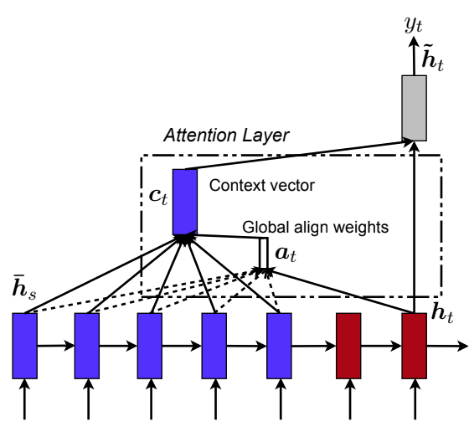
\includegraphics[width=10cm]{images/global.png}
\centering
\caption{An RNN architecture with global attention: all first-layer hidden states are used to construct an output. \parencite{Luong2015}}
\label{fig:global}
\end{figure}

\begin{figure}[p]
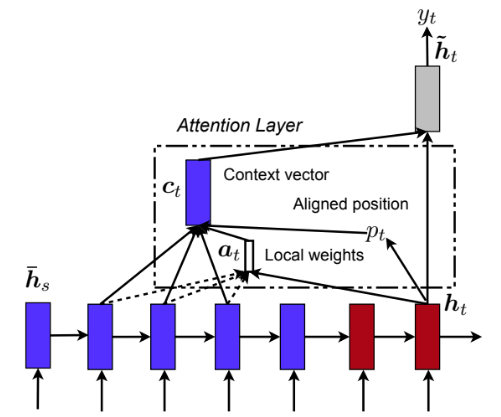
\includegraphics[width=10cm]{images/local.png}
\centering
\caption{An RNN architecture with local attention: only a subset of hidden states, not necessarily contiguous, are used to construct an output. \parencite{Luong2015}}
\label{fig:local}
\end{figure}

The main differences between the LSTM architectures used in state of the art applications now, as evidenced by the four architectures used as baselines in the SIGMORPHON 2019 transfer learning task, are in their \textbf{attention mechanism}, the means by which hidden states are combined to generate sequential output \parencite{Cotterell2019}. 

The main contrasting terminologies for attention are \textbf{hard} vs. \textbf{soft}, and \textbf{global} vs. \textbf{local}. In soft attention models, hidden states are all considered, weighted using an additional layer. In hard attention models, only a limited subset of hidden states are considered, the selection of hidden states may be chosen by the model at each stage or consist of a single sliding window of attention. Soft attention models are straightforward to apply backpropagation to, since each hidden state has a differentiable relationship to the output, while hard attention models that select which hidden states are used at a particular time step are not. A \textbf{monotonic} hard attention model is one in which the window of attention moves through the input at the same rate that the output is generated, which is applicable in scenarios when corresponding positions in input and output are expected to be strictly related. \textbf{Global} vs. \textbf{local} attention refers to whether all or only a narrow range of hidden states contribute to a hard attentional layer, as depicted in Figs. \ref{fig:global} and \ref{fig:local} \parencite{Luong2015}. 

\section{Transfer learning}

Transfer learning is a high-level term for any machine learning process for which either the domain or the distribution of some or all training data inputs is different from that of the inputs to which a model will ultimately be applied. Such techniques arise in response to the conundrum that many real-world machine learning problems face: a lack of data that looks like the system that one wishes to predict or understand, either due to insufficient available quantity, or altogether lack in the case of seeking to predict the outcome of future events of which no past equivalents exist. The machine learning problem for which a model is initially trained is called the \textbf{source task}; the problem which the model is being constructed to solve is called the \textbf{target task}. Typically, the source model is not the only component of the eventual target model - manual output transformations or additional machine learning is usually applied \parencite{Pan2010}.

\begin{figure}[t]
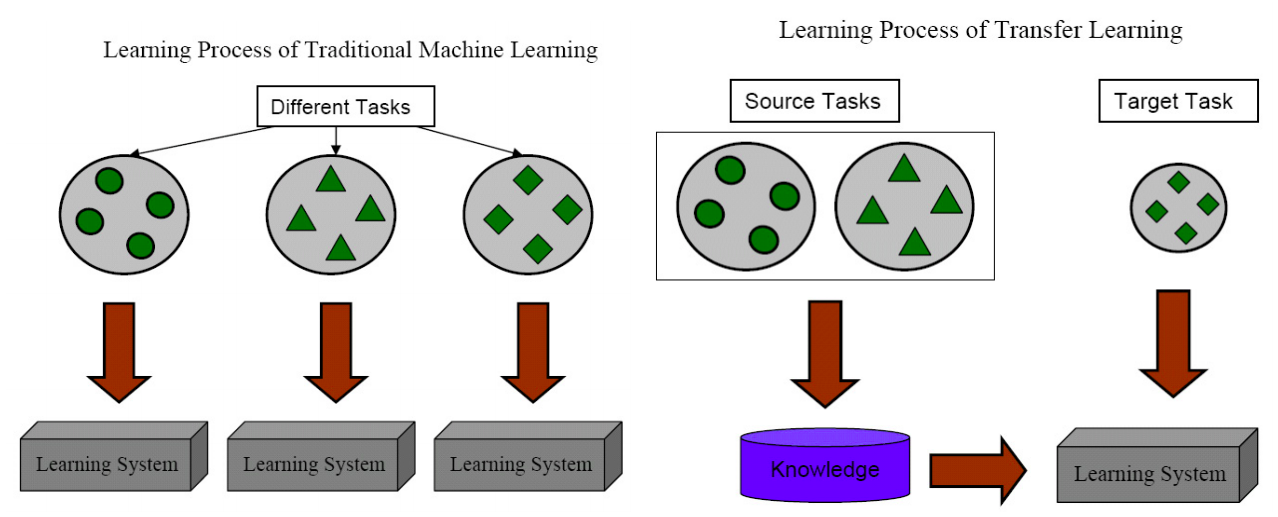
\includegraphics[width=12cm]{images/transfer_learning.png}
\centering
\caption{An abstract characterization of traditional ML vs. transfer learning}
\end{figure}

Some examples are provided by Pan and Yang 2010. One is the problem of seeking to classify web documents by topic. If a significant portion of the documents that will need to be classified bear on topics rarely covered in an existing corpus of web documents, this is an example where the training and test domains are roughly similar but their distribution is different; it is perhaps a less obvious transfer learning problem. Another example is that of attempting to gauge sentiment of reviews of cameras, when the only available data is a corpus of reviews of other types of products. In this case, knowledge of many domains, none of which is equal to the target domain, must be transferred to attempt to make predictions about the target domain.

There are three broad categories of transfer learning that Pan and Yang identify, which differ in their intrinsic difficulty. \textbf{Inductive transfer learning} describes a modeling scenario in which the domains of source and target are identical, but the target task is different, that is, the codomain of the model differs. In inductive transfer learning, output from the source model is used to inform a model of the target task. \textbf{Transductive transfer learning} describes the scenario that the task is the same but the source and target domains are in some way different, either differing in feature space, or having the same feature space but differing in distribution over that space. The two examples above are both instances of transductive transfer learning; the web document categorization problem is an example of differing distribution while the review sentiment analysis problem is an example of differing feature space. \textbf{Unsupervised transfer learning} describes the scenario that source and target differ in both domain and codomain. 

An example of unsupervised transfer learning is the morphology transfer learning problem that this thesis undertakes: labeled training inputs and outputs from the source (one language) are used to inform a model of the target task (a different language), and the feature spaces of both domain (lexemes and morphological categories) and codomain (inflected forms) differ between the two. After all, no two languages share the same set of words, and only in the case of very closely related languages or extreme coincidence will all grammatical paradigms inflect for the same set of morphological categories (one language is likely to have a grammatical gender, a verb tense, or some other category that the other language lacks).

There is precedent for transfer learning on LSTMs for language technology tasks, typically with the explicit goal of dealing with low data volume in the target task due to sparse language resources. The baseline for SIGMORPHON 2019 was based on the LSTM transfer learning architecture introduced in Zoph et al. 2016 \parencite{McCarthy2019}, which was applied there to a transductive machine translation task. Their approach is relatively straightforward - they use an LSTM encoder-decoder model to train a machine translation system from French to English on a high data volume, then use that model as the initialization of an architecturally identical Uzbek-English model, holding the decoder fixed and simply allowing the encoder to learn encodings for Uzbek with quite a small dataset. Their results showed considerable improvements over similarly low-data machine translation techniques \parencite{Zoph2016}, suggesting that transfer learning may be a promising strategy for computational linguistics tasks.

\section{Ensembling}

\textbf{Ensembling} is another core ML concept that arises in explaining the differences in structure and performance of computational morphology models. It is a generic term for combining the outputs of multiple models which operate over the same domain and codomain. That is, ensembled models receive the same input, and produce outputs of the same form; their outputs are typically combined by vote in classification tasks or weighted or unweighted averaging in regression tasks. Ensembling among neural and non-neural models has been used to improve outcomes in a variety of tasks \parencite{Krogh1995}.

\chapter{Machine learning of morphology: existing work}

\section{Sub-problems and related problems}

Within the realm of machine understanding of morphology, there are many sub-problems and related problems. The most basic areas of research involve predicting the inflection morphology of words in isolation - transforming a word into a specific morphological form, or the inverse, tagging a form with its morphological categories. 

In this section, I used the machine learning terms \textbf{supervised} and \textbf{unsupervised}. Supervised learning is that conducted with labeled input-output sets, in which a model attempts to produce outputs similar to those it's seen. Unsupervised learning is that which attempts to find patterns in data sets with no output, such as finding clusters in a scatter plot of points. Note that this definition of \textbf{unsupervised} differs from the sense specific to transfer learning. The transfer learning task in SIGMORPHON 2019 is an example of an \textit{unsupervised} transfer learning problem in that the source domain and codomain are both different from target domain and codomain, yet it is \textit{supervised} in a general ML sense in that the triples included in the training data include output values which the model attempts to mimic.

\subsection{Core supervised learning problems}

Some of the earliest work in computational morphology involves making specific morphological transformations. That is, given a particular form of a lexeme (often, but not necessarily, a citation form), predicting another form. An example would be learning to transform English verbs from present to past tense, e.g., \textit{show} $\rightarrow$ \textit{showed}, \textit{see} $\rightarrow$ \textit{saw}, etc. \parencite{Dreyer2008}.

The natural extension of this is aiming to be able to predict any inflected form given one specific form of a lexeme and an arbitrary set of morphological categories. For instance, given a lexeme \textit{see} and the categories \texttt{3rd person singular, simple present}, generating the correct form \textit{sees}. Generally speaking, a citation form has been used as input (\cite{Durrett2013}, \cite{Faruqui2015}, \cite{Cotterell2017a}). The related "reinflection" problem involves being given any inflected form as input, and transforming it into any other \parencite{Cotterell2016}.

A further extension of the morphology generation problem is the generation of complete inflection tables. The exact nature of this problem depends on the type of training and test data used. If a model is only trained on a sparse, random sampling of forms for each lexeme, then a task may consist of filling out the rest of an inflection table for those lexemes. For instance, a model may be given the forms \textit{sees} and \textit{seeing} among its training data, and be required to fill out the remaining forms of that paradigm, including \textit{see} and \textit{saw}. If a model is instead trained using entire inflection tables, e.g., all forms of the verb \textit{see}, then test data must consist of new lexemes (\cite{Hulden2014}, \cite{Ahlberg2015}, \cite{Cotterell2017a}).

\subsection{Inflection types}

Overall, a diverse set of inflection shapes have been worked with in the most recent efforts of this subfield. Since 2016, the Special Interest Group on Computational Morphology and Phonology (SIGMORPHON), a research collective focused on computational morphology and related problems, has fielded "shared tasks" in which several research teams globally are given training data and a task definition, and attempt to create models which are subsequently compared. The SIGMORPHON shared task 2018 included training data from 103 typologically diverse languages, and paradigms using suffixing, prefixing, infixing, reduplication, and non-concatenative morphology. 

\subsection{Related problems}

Within only the last two or so years, there has been work on predicting morphology in context. In the 2018 and 2019 SIGMORPHON shared tasks, to which several teams of researchers submitted solutions, a sub-task was dedicated to cloze challenges, a type of test in which one word in a sentence, given in citation form, was to be inflected based on context (\cite{Cotterell2018b}, \cite{McCarthy2019}). This work is essentially a synthesis of morphology generation and morphosyntactic modeling.

Since 2017, there has been some work done on learning curves for computational morphology. The datasets published for SIGMORPHON 2017 and 2018 include partitions into low ($\sim$100 forms), medium ($\sim$1000 forms), and high ($\sim$10,000 forms) data training sets for the express purpose of assessing the learning curve of different models. Evidence suggests that learning curve varies by model type. LSTMs are generally the most accurate morphology models with high-data training sets and are considered state of the art. However, LSTMs and related neural model types often fare worse than more baseline string transduction models with small training sets, likely due to the very gradual gradient descent process used to fine-tune them (\cite{Cotterell2017a}, \cite{Cotterell2018b}). Improving performance with small training sets is of interest, as much of the applicability of computational morphology models is to languages which don't already have high-quality technical tools or datasets. 

The most recent new challenge that SIGMORPHON has tried to address is that of transfer learning of morphology, in the shared task earlier this year. Given a state of the art model trained on a language with a high volume of training data, teams were asked to alter it into a model that would perform well on a new language, given a smaller amount of training data for that language. 80\% of the pairs of languages were closely related, while 20\% were distantly or not at all related. Gains of transfer learning models between closely related languages were said to have generally performed better than transfer learning models between more distant languages \parencite{McCarthy2019}, although that conclusion is be examined more closely in this study.

\section{Non-neural approaches}

\subsection{Vector embedding}

A technique that has found success in a variety of computational linguistics tasks is that of representing words in relatively low-dimensional vector spaces. That is, words are represented as a vector, a series of numbers of fixed length; the length of the vector is typically much smaller than the number of total known words. This has the intention of capturing semantic and syntactic content in a principled way - similarities between the numbers representing two words are expected to signify actual similarity in their meaning, and regular linear transformations between vectors should roughly correspond to specific semantic or grammatical changes. These vector representations can be generated via various unsupervised learning methods (\cite{Bilmes2003}, \cite{Alexandrescu2006}).

\begin{figure}[ht]
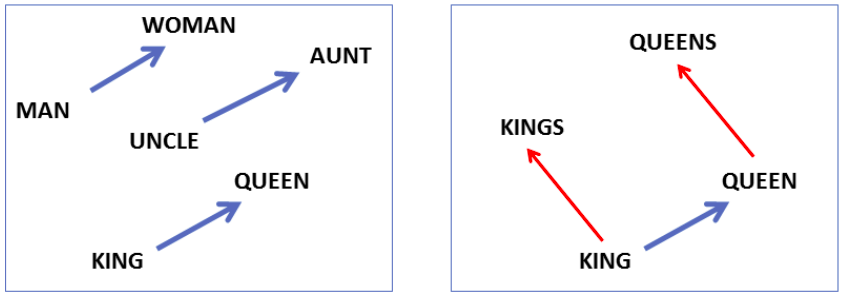
\includegraphics[width=12cm]{images/semantic_transform.png}
\centering
\caption{Regular spatial transformations encode semantic or grammatical content \parencite{Mikolov2013}}
\label{fig:vectors}
\end{figure}

Regularities in the relative location of semantically related words have been exploited for semantic analysis tasks \parencite{Alexandrescu2006}. Similarly, morphological changes may appear as spatial transformations in vector space, and work has been done on discovering morphological relationships between in-vocabulary words based on their relative spatial locations (\cite{Mikolov2013}, \cite{Soricut2015}, \cite{DosSantos2014}). Fig. \ref{fig:vectors}  illustrates this idea in a slightly simplified way: once a vector embedding model has been trained on English, it can be discovered that semantic transformations (male to female) and grammatical transformations (singular to plural) roughly correspond to regular spatial translations in vector space.

Vector embedding has the limitation that it cannot extend to words for which a vector representation has not been trained, and so it cannot directly provide understanding of the many OOV forms encountered in test data of highly inflected languages (\cite{Soricut2015}, \cite{Cotterell2019}). However, it can be a means to discover relationships between words in an unsupervised manner, which may support labeling tasks in support of computational morphology and other tasks.

\subsection{String transduction}

Earlier work specifically focused on the problem of morphology prediction made use of iteratively improving methods of string transduction - in essence, pattern matching on the written representations of words (\cite{Durrett2013}, \cite{Hulden2014}, \cite{Nicolai2015}, \cite{Ahlberg2015}). Typical steps of string transduction methods include character alignment (depicted in Fig. \ref{fig:chalign}), identification of characters that are inserted or deleted based on grammatical form, and generalization of lexemes which are inflected by the same sets of insertions or deletions (depicted in Fig. \ref{fig:transduction}). 

\begin{figure}[ht]
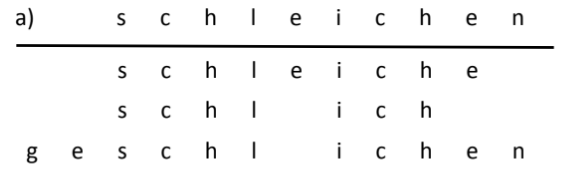
\includegraphics[width=12cm]{images/Nicolai2015_schleichen.png}
\centering
\caption{Character alignment for various forms of the German verb \textit{schleichen} \parencite{Nicolai2015}.}
\label{fig:chalign}
\end{figure}

\begin{figure}[ht]
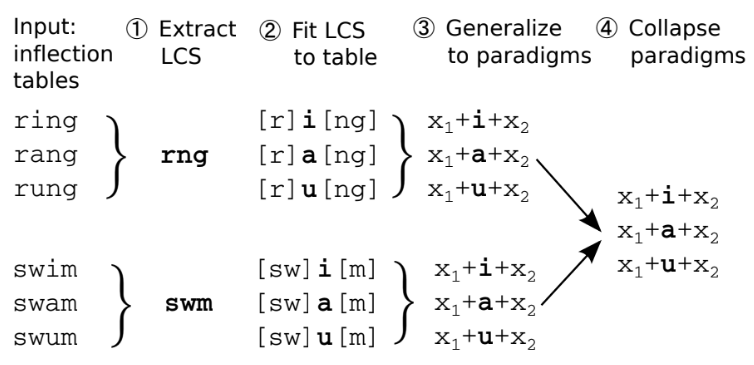
\includegraphics[width=12cm]{images/Hulden2014_diagram.png}
\centering
\caption{Conceptual depiction of a typical example of a string transduction method of morphology learning \parencite{Hulden2014}.}
\label{fig:transduction}
\end{figure}

A crucial limitation of string transduction methods are their general assumption that most lexemes have exactly the same set of characterwise transformations as a large group of other lexemes, and that a manageably small number of such inflection classes exist. There are paradigms with such a limited set of inflection classes, such as Spanish \textit{-ar}, \textit{-er}, and \textit{-ir} verbs. However, when multiple morpholonological processes are at play, individual lexemes may be nearly unique in their exact set of transformations.

For example, Finnish noun declension has processes of vowel harmony, consonant gradation, and vowel alternation and lengthening operating to produce final inflected forms \parencite{Ranta2008}. As an illustration, consider the Finnish nouns \textit{puku} "suit" and \textit{kenkä} "shoe", which have the inessive singular forms \textit{puvussa} "in the suit" and \textit{kengässä} "in the shoe", respectively. In both forms, the letter \textit{k} is transformed via consonant gradation, but the letter it becomes depends on the surrounding letters. The final vowel of the forms may be \textit{a} or \textit{ä}, depending on vowel harmony. In other inflected forms, the final vowel of the words may be doubled \parencite{Wiktionary}. A model that naively seeks to match these words with other words using the same set of character transformations across the paradigm may need to assign nearly every word to its own category, failing to generalize the patterns at work.

The poorer performance of string transduction relative to neural models has led to a move of the field away from string transduction since about 2016 \parencite{Cotterell2018b}.

\section{LSTM and other neural approaches}

Since 2016, almost all work on paradigm completion has made use of long short-term memory (LSTM) or related gated recurrent network (GRU) models (\cite{Faruqui2015}, \cite{Cotterell2016}, \cite{Cotterell2017a}, \cite{Cotterell2018b}, \cite{McCarthy2019}). An LSTM network is a variation on a recurrent neural network (RNN), a variant of neural network \parencite{Hochreiter1997}.

The SIGMORPHON 2019 transfer learning task used a diverse set of architectures as baselines, including a soft attention, a non-monotonic hard attention, and two monotonic hard attention models, reflecting a diversity of strategies employed by the best current models. Soft attention has dominated prior morphology learning work, but Wu and Cotterell (2019) demonstrate that hard monotonic models may be more appropriate for morphology tasks, where string transductions are mostly monotonic - that is, (except for in instances of reduplication or metathesis) characters in an input word correspond to characters in the same order in the output (\cite{McCarthy2019}, \cite{Wu2019}).

\section{Ensembling approaches}

\begin{figure}[ht]
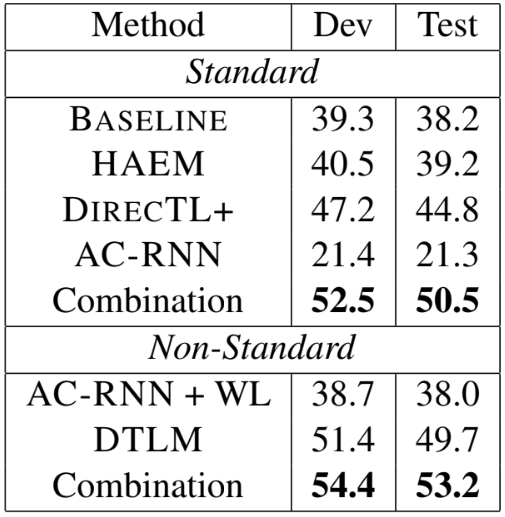
\includegraphics[width=7cm]{images/Najafi_accuracy.png}
\centering
\caption{The low-resource accuracy scores of the various University of Alberta models submitted to SIGMORPHON 2018 \parencite{Najafi2018}.}
\label{fig:Najafi}
\end{figure}

Ensembling was used in SIGMORPHON 2018 by various groups between neural and non-neural methods, specifically to ameliorate the poor performance of neural models in low-data settings \parencite{Cotterell2018b}. For example, the University of Alberta submission \texttt{UA-05} uses weighted voting to combine the 2019 baseline, a hard-attention LSTM model, a soft-attention LSTM model, and a string transduction model, favoring the output of generally more accurate models unless other models can agree on a different output. The \texttt{UA-08} system submitted by the same team combines the output of a string transduction and a soft-attention LSTM in a totally different way, by linear combination of their self-determined confidence scores \parencite{Najafi2018}.

Fig. \ref{fig:Najafi} shows the accuracy scores of the UA models averaged over all 103 languages of SIGMORPHON 2018 in the low-resource setting. \textsc{DirecTL+} and \textsc{DTLM} are string transduction models, \textsc{Baseline}, HAEM, AC-RNN, and AC-RNN + WL are LSTM models, and the two combinations are \texttt{UA-05} and \texttt{UA-08}, respectively; notice that the string transduction models score higher accuracy than neural models, but both ensembling methods have the highest accuracy of all.